\emph{Type Checking} is the process used for the verification of types constraints:
\begin{itemize}
    \item
    can be performed at compiling time (static check) or at execution time (dynamic check);
    \item
    dynamic types appear more often in interpreted languages, whereas compiled languages favour static types;
    \item
    static checking is one of the main semantic tasks performed by a compiler.
\end{itemize}
\subsubsection{Type Systems}
\begin{description}
    \item[Base Types]
    Programming languages typically include base types for numbers, characters, and boolean.
    \item[Compound and Constructed Types]
    Programmers need higher level abstractions than the base types.
    Programming languages provide mechanisms to combine and aggregate objects and to derive types for the resulting objects.
\end{description}
A type system consists in a set of base types and a set of type constructors.
Using base types and type constructors each expression in a program can be represented with a type expression.

\section{Type Expression}
Generally, types can be divided in:
\begin{itemize}
    \item
    primitive types;
    \item
    composite types.
\end{itemize}
Primitive types comprise all the types necessary to formalization of a given language (e.g., \emph{int}, \emph{float}, \emph{char}) together with two special ones:
\begin{description}
    \item[void]
    stating the absence of a type;
    \item[type-error]
    stating an error found during the type checking phase.
\end{description}

A \emph{type expression} is either a base type or is formed by applying a type constructor to a type expression.

\subsection{Type Constructors}
Examples referred to the C language:
\begin{description}
    \item[array]
    $array(I,T)$ ($I$: size of the array, $T$: type expression)
    \item[pointers]
    $pointer(T)$
    \item[product]
    $T_1 \times T_2$
    \item[structures]
    $struct(T)$
\end{description}
\begin{table}[h]
    \centering
    \begin{tabular}{l|l}
        Declaration & Type Expression \\ \hline
        \code{char v[10]} & $array(10, char)$ \\ \hline
        \code{struct\{ int i; char s[5]\} } & $struct((i \times int) \times (s \times array(5, char)))$ \\
    \end{tabular}
\end{table}

\subsubsection{Functions}
A function maps an element of its own domain to an element in its own range.

Functions $T_1 \to T_2$ ($T_1$: domain type, $T_2$:range type)

The function \code{int * F(char a, char b)} is represented using the following type expression: $(char \times char) \to pointer(int)$

\subsection{Types Graph}
An effective way of representing type expressions consists in the use of graphs (trees or DAGs).
Example: $(char \times char) \to pointer(int)$

\subsubsection{Tree}
\begin{figure}[H]
    \centerline{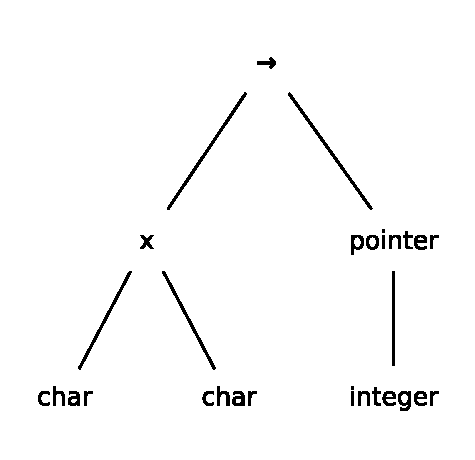
\includegraphics[width=0.3\textwidth]{img/36.pdf}}
\end{figure}

\subsubsection{DAG}
\begin{figure}[H]
    \centerline{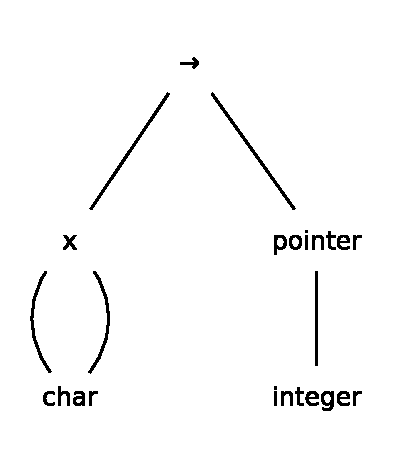
\includegraphics[width=0.3\textwidth]{img/37.pdf}}
\end{figure}

\subsection{Constructions of Type Expressions}
A type checker for the C language could be implemented by means of the following grammar and semantic rules:
\begin{table}[H]
    \centering
    \begin{tabular}{l|l}
        $D \to T \; VL \; ';'$ & \code{VL.type = T.type} \\ \hline
        $VL \to V$ & \code{V.type = VL.type} \\ \hline
        $VL \to VL_1 \; ',' \; V$ & \code{V.type = VL.type} \\ \hline
        $V \to '\ast' \; V_1$ & \code{V1.type = pointer(V.type)} \\ \hline
        $V \to VA$ & \code{VA.type = V.type} \\ \hline
        $VA \to VA_1 \; '[' \; num \; ']' $ & \code{VA1.type = array(num.val, VA.type)} \\ \hline
        $VA \to ID$ & \code{add_var(ID.name, VA.type)} \\
    \end{tabular}
\end{table}
\begin{figure}[H]
    \centerline{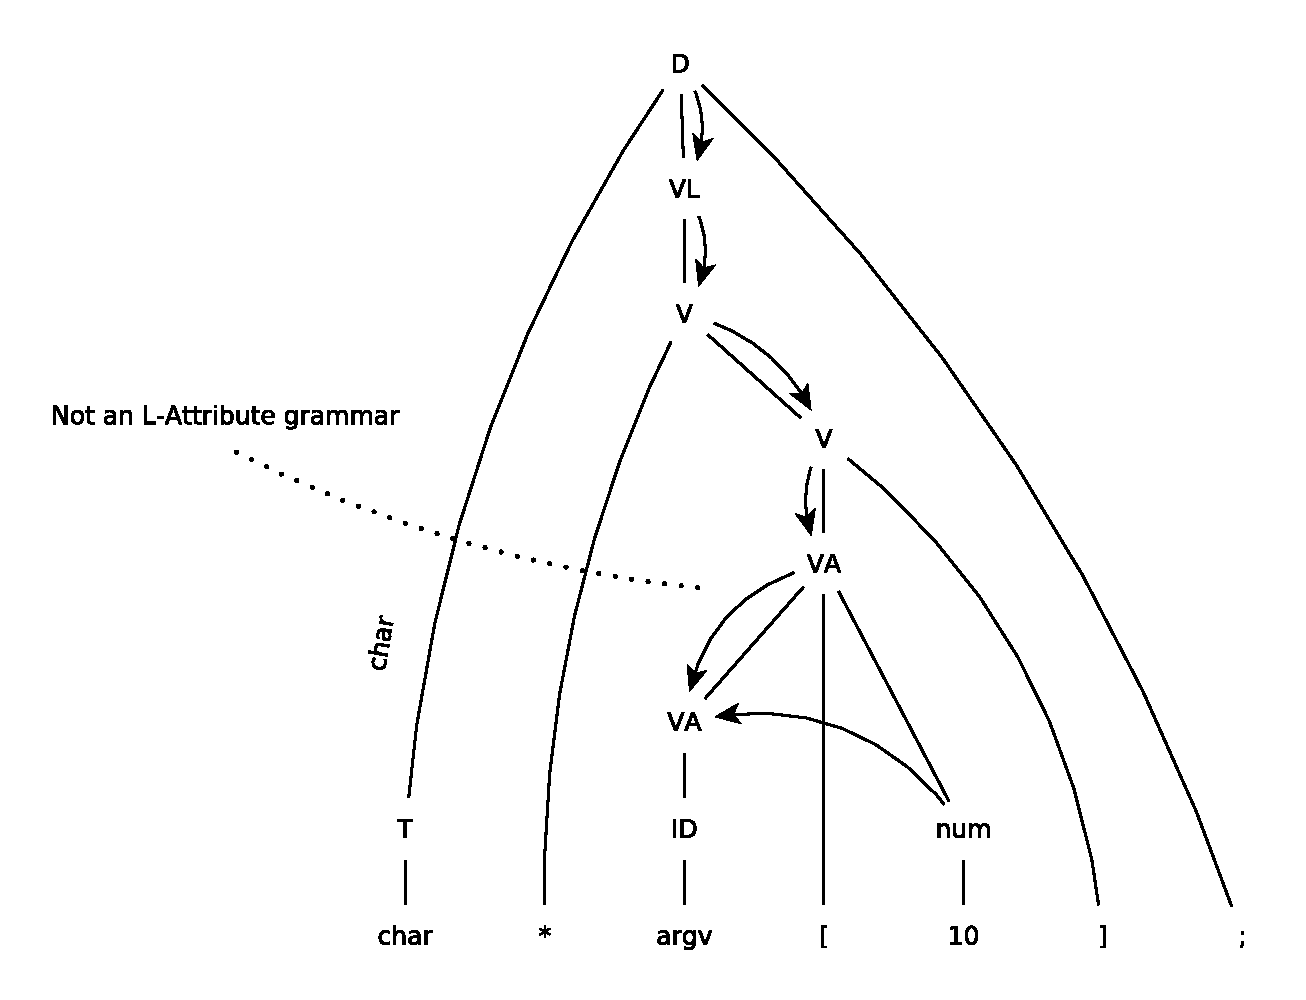
\includegraphics[width=1\textwidth]{img/38.pdf}}
\end{figure}
\subsubsection{Fix}
\begin{table}[H]
    \centering
    \begin{tabular}{l|l}
        $D \to T \; VL \; ';'$ & \code{VL.type = T.type} \\ \hline
        $VL \to V$ & \code{V.type = VL.type} \\ \hline
        $VL \to VL_1 \; ',' \; V$ & \code{V.type = VL.type} \\ \hline
        $V \to P \; ID \; A$ & \code{P.base = V.type} \\
        & \code{A.base = P.base} \\
        & \code{add_var(ID.value, A.type)} \\ \hline
        $P \to \varepsilon$ & \code{P.type = P.base} \\ \hline
        $P \to P_1 \; '\ast'$ & \code{P.type = pointer(P1.type)} \\
        & \code{P1.type = P.base} \\ \hline
        $A \to \varepsilon$ & \code{A.type = A.base} \\ \hline
        $A \to A_1 \; '[' \; num \; ']' $ & \code{A.type = array(num.val, A.type)} \\
        & \code{A1.type = A.base} \\
    \end{tabular}
\end{table}

\subsection{Types Names}
In many languages it is possible to assign explicit names to types; examples:
\begin{table}[H]
    \centering
    \begin{tabular}{l|l}
        \code{typedef cell * link} & \code{type link = ^cell;} \\ \hline
        \code{link p} & \code{var p: link;} \\ \hline
        \code{cell * q} & \code{var q: ^cell;} \\ \hline
    \end{tabular}
\end{table}
Do variables \code{p} and \code{q} belong to the same type?
Answer depends on the approach used to check them.

\subsection{Name Equivalence}
Two expressions are equivalent if:
\begin{itemize}
    \item
    they belong to the same primitive type;
    \item
    they are based on the application of the same type constructors to equivalent types.
\end{itemize}

Using a tree-based representation for type expression it is possible (and convenient) to use a recursive visit algorithm in order to verify the equivalence.

\subsection{Type Checker}
A \emph{type checker} comprises a set of interoperating modules:
\begin{description}
    \item[scanner]
    lexicon recognition;
    \item[parser]
    checks the syntax and adds the semantic;
    \item[type expression manager];
    \item[symbol table manager].
\end{description}
\begin{figure}[H]
    \centerline{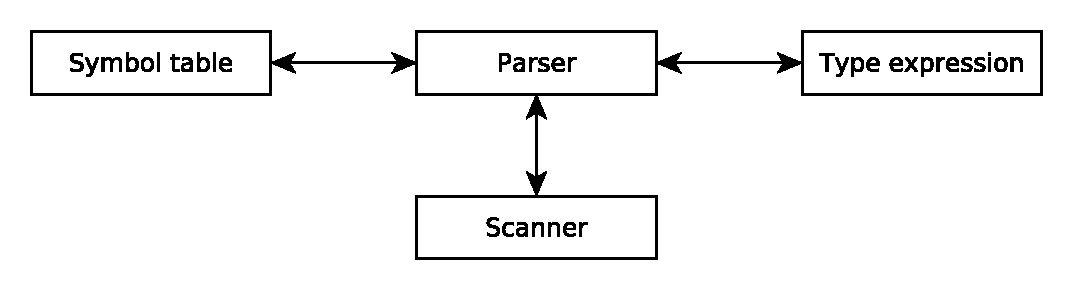
\includegraphics[width=0.8\textwidth]{img/39.pdf}}
\end{figure}

\section{Symbol Table}
Symbol tables associate values to names in order to make accessible the semantic information related to an identifier outside of the context where it has been declared.
Information related to each name is used in order to verify the semantic correctness of identifiers usage within a program.
Such information is dynamically updated as new features of the identifier and declared in the program of inferred by the compiler.

Single pieces of information stored within a symbol table are named \emph{entry}.
Each introduction operation defines a key (usually a \code{String}) by which it is possible to retrieve (later) the desired information.
Usually, the entries within a table are not homogeneous therefore it is more convenient to use pointers instead of the entries themselves.

A translator uses different symbol tables in order to store information pertaining to different contexts.

\subsection{Designing a Symbol Table}
A symbol table can be implemented by using different data structures:
\begin{itemize}
    \item
    unordered list;
    \item
    ordered list;
    \item
    binary tree;
    \item
    hash table;
    \item
    btree.
\end{itemize}
This choice is based on the number of symbols to store, on the required performances, and on the complexity of the code to be produced.

Example:
\begin{lstlisting}[frame=single]
import java.util.HashTable;

// Initialize the table
HashTable symTable = new HashTable();

// Insert entries: int a, float b
symTable.put("a", "int");
symTable.put("b", "float");

// Get value of "a"
String type = (String) symTable.get("a");
System.out.println(type);

// Delete entry
symTable.remove("a");

// Clear the table
symTable.clear();
\end{lstlisting}

\subsection{Type Expression}
Type expressions (naturally represented by means of trees of types) can be transformed into a different internal representation (i.e., Java class).
The management of type expressions requires:
\begin{itemize}
    \item
    the definition of the data structures associated to each graph node;
    \item
    the definition of primitives that operate on node.
\end{itemize}
Nodes should be capable of representing the different type constructors and the base types as well.
Primitives are required in order to hide the internal representation of nodes thus allowing the user to produce the easiest code possible.

\subsubsection{Implementing Type Expressions}
Each node of a type graph comprises:
\begin{itemize}
    \item
    a tag, representing the type of node;
    \item
    a set of different fields depending on the type of data to be stored.
\end{itemize}

\begin{lstlisting}[frame=single]
public class TENode {
    public int tag; // base, array, pointer, ...
    public int size; // number of elements in array
    public int code; // base type: int, char, float

    // only for structs
    public String name; // struct name

    // left and right children
    private TENode left, right;
}
\end{lstlisting}
The module in charge to manage type expressions should offer the following primitives:
\begin{lstlisting}
public static TENode teMakeBase(int code);
public static TENode teMakePointer(TENode base);
public static TENode teMakeArray(int size, TENode base);

// only for structs and functions
public static TENode teMakeProduct(TENode l, TENode r);
public static TENode teMakeName(String name);
public static void teConsStruct(TENode str, TENode flds);
public static TENode teMakeFwdStruct(String name);
public static TENode teMakeStruct(TENode flds, String n);
public static TENode teMakeFunction(TENode d, TENode r);
\end{lstlisting}

\section{Type Checker}
\subsection{Semantic}
In addition to the primitives offered by the type expression module, it is a good practice providing primitives to access the symbol tables
\begin{itemize}
    \item
    if the recognition of structs is required:
    \begin{itemize}
        \item
        \code{int addType(String name, TENode type);}
        \item
        \code{TENode typeLookup(String name);}
    \end{itemize}
    \item
    always:
    \begin{itemize}
        \item
        \code{int addVar(String name, TENode type);}
    \end{itemize}
\end{itemize}
Besides simplifying the code of semantic actions, such primitives allow to hide implementation details of tables.

\subsection{Complete Grammar}
\begin{lstlisting}[frame=single]
S ::=
    | S decl ';';

decl ::= T vList
    | typedef T ID;

T ::= type
    | struct ID '{' sfl '}'
    | struct '{' sfl '}'
    | struct ID;

sfl ::= field
    | sfl field;

field ::= T vList;

vList ::= V
    | vList ',' V;

V ::= ptr ID array;

ptr :=
    | ptr '*';

array ::=
    | array SO num SC;
\end{lstlisting}

\subsection{Semantic}
\begin{lstlisting}[frame=single]
decl ::= T vList;

T ::= type:t {: RESULT = (TENode) t; :};

vList ::= V:t {: RESULT = (TENode) t; :}
    | vList:t ';' {: RESULT = (TENode) stack[top - 1]; :}
    | V {: RESULT = t; :};

V ::= ptr ID:a arr:t {:
    addVar(a, t);
    RESULT = (TENode) stack[top - 3];
:};

ptr ::= {: RESULT = (TENode) stack[top]; :}
    | ptr:p '*' {: RESULT = teMakePointer(p); :};

arr ::= {: RESULT = (TENode) stack[top - 1]; :}
    | arr:a SO num:b SC {: RESULT = teMakeArray(b, a); :};
\end{lstlisting}